% Section content template for individual Educative lessons
% This file contains the actual content for a specific section
% Generated from Educative API section content

% Section: Resources to Prepare for a System Design Interview
% Section ID: 5546916426809344
% Section Slug: resources-to-prepare-for-a-system-design-interview
% Generated: 2025-08-02T19:56:31.057845

\noindent
\begin{minipage}[t]{0.48\textwidth}
Substantial preparation is necessary to increase our odds of getting the job we apply for. Depending on a candidate's seniority and proficiency, different candidates need different times for interview preparation. For an average candidate, three to four months might be required to prepare for a System Design interview.
\end{minipage}
\hfill
\begin{minipage}[t]{0.48\textwidth}

\includegraphics[width=0.8\textwidth]{Images/chapter_1/section_5546916426809344/5699614642929664.png}
\end{minipage}

\noindent
\begin{minipage}[t]{0.48\textwidth}

\end{minipage}
\hfill
\begin{minipage}[t]{0.48\textwidth}

\end{minipage}

\subsection{This course}\label{7xxiaspEOx6hDBiwP4TQV}

This course helps readers learn or brush up on their system design skills. We 've carefully curated some traditional and fresh design problems to cover the substantial depth and breadth of the system design. The following activities might expedite the preparation and add variety and further depth to a candidate's knowledge.

\subsection{Technical blogs/System Design interview articles}\label{AVkodIpO9v5zZuv5hm-2f}

Many companies regularly publish the technical details of their significant work in the form of technical blogs.

\begin{figure}[htbp]
 \centering
 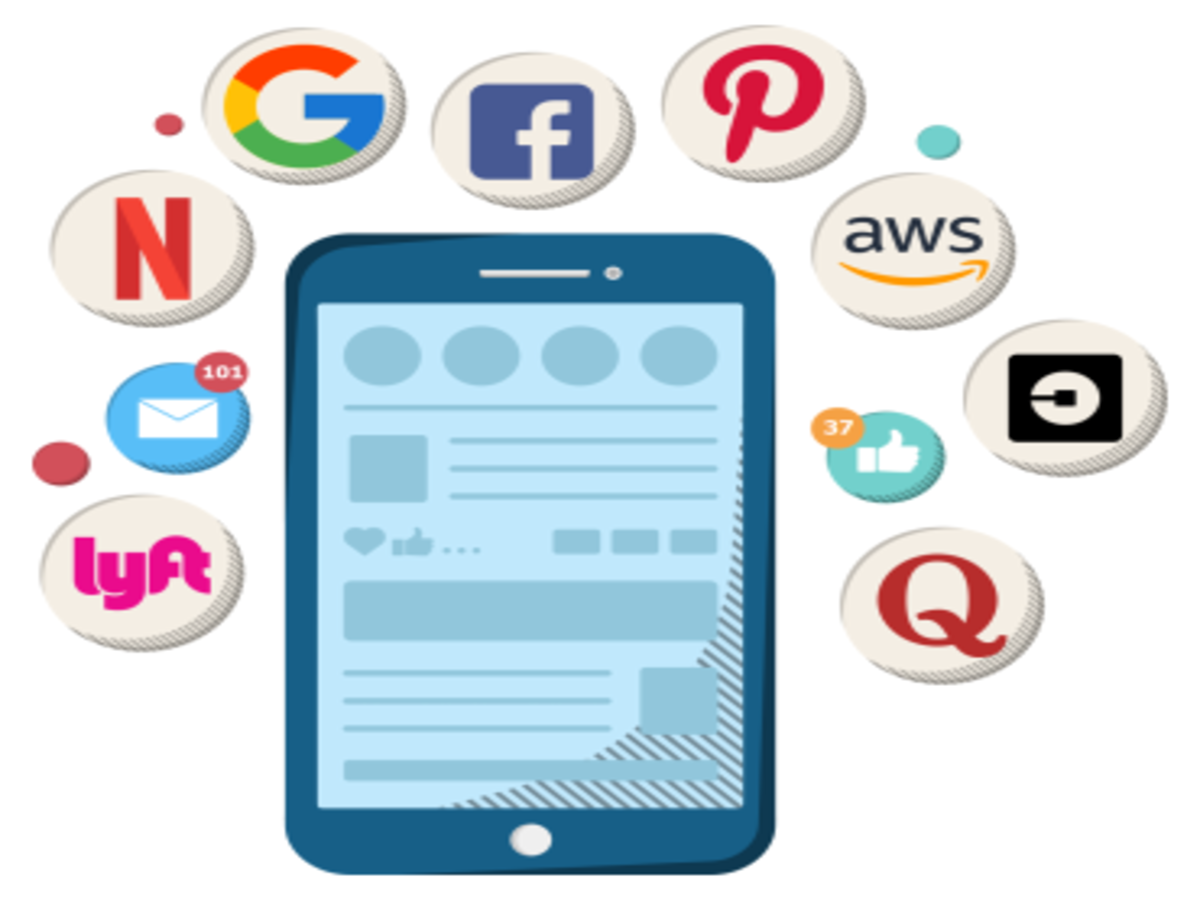
\includegraphics[width=0.8\textwidth]{Images/chapter_1/section_5546916426809344/4830700849463296.png}
 
\end{figure}

\begin{quote}
\textbf{Quiz:}
\textbf{Question 1:} Why are companies eager to share the technical details of their work?
\textbf{Answer:} The reason for such sharing is to excite the technical community about the fact that the company is solving hard problems. They also hope to motivate more people to join their company. Such public blogs can also help to advertise company products to B2B customers. Additionally, such material helps the company train potential future workers on their own time. Lastly, the main reason is to let the learner know that the company has deep expertise in the specific domain or subject matter.
\end{quote}

\begin{quote}
\textbf{Note:}~There's a fine line between what can be held back by a company due to a competitive edge and what can be made public.
\end{quote}
We can study these blogs to gain insight into the company's challenges or problems and the changes it made in the design to cope with them.
\begin{quote}
\textbf{Note:}~Staying informed about these innovations is important for professionals, and even more crucial for an applicant.
\end{quote}
Some important technical blogs are~\href{https://engineering.fb.com/}{Engineering at Meta},~\href{https://research.fb.com/}{Meta Research},~\href{https://aws.amazon.com/blogs/architecture/}{AWS Architecture Blog},~\href{https://www.amazon.science/blog}{Amazon Science Blog},~\href{https://netflixtechblog.com/}{Netflix TechBlog},~\href{https://research.google/}{Google Research},~\href{https://quoraengineering.quora.com/}{Engineering at Quora},~\href{https://eng.uber.com/}{Uber Engineering Blog},~\href{https://databricks.com/blog/category/engineering}{Databricks Blog},~\href{https://medium.com/@Pinterest_Engineering}{Pinterest Engineering},~\href{https://medium.com/blackrock-engineering}{BlackRock Engineering},~\href{https://eng.lyft.com/}{Lyft Engineering}, and~\href{https://engineering.salesforce.com/}{Salesforce Engineering}.

We at Educative are open to sharing technical knowledge with our learners. Our comprehensive repository of blogs comprises interview prep guides, FAANG-specific insights, and in-depth technical blogs. FAANG-specific System Design interview articles include \href{https://www.educative.io/blog/google-system-design-interview-questions}{Google}, \href{https://www.educative.io/blog/microsoft-system-design-interview}{Microsoft,} \href{https://www.educative.io/blog/netflix-system-design-interview-questions}{Netflix,} \href{https://www.educative.io/blog/amazon-system-design-interview}{Amazon,} and \href{https://www.educative.io/blog/meta-system-design-interview}{Meta}.

A few other guides and articles related to technical concepts are given in the following sections.

\subsubsection{System Design interview guides}\label{AE9oW82se-gKKdMCDZXZp}

\begin{itemize}
\item
\phantomsection\label{jn-BA-j6sT4X-8k1q9C4W}
\href{https://www.educative.io/blog/faang-system-design-interview-guide}{A beginner's guide to System Design Interviews at FAANG/MAANG}
\item
\phantomsection\label{jQZbauZ1NJ5njnFtYpqxf}
\href{https://www.educative.io/blog/system-design-interview-expert-tips}{System Design interview guide: Tips from an industry expert}
\item
\phantomsection\label{LRuuB1_medp_4cpJ_y698}
\href{https://www.educative.io/blog/use-reshaded-for-system-design-interviews}{Simplify System Design interviews with the RESHADED approach}
\end{itemize}

\subsubsection{System Design interview technical insights}\label{CBnAOeV_MLYXgoifMvrKW}

\begin{itemize}
\item
\phantomsection\label{5H4-hsVGCjTXZstJgj5ns}
\href{https://www.educative.io/blog/system-design-interview-questions}{25 essential System Design Interview Questions in 2024}
\item
\phantomsection\label{K4DTFO3Wrs7eeMbNtjJMT}
\href{https://educative.io/blog/system-design-caching}{A complete guide to System Design caching}
\item
\phantomsection\label{zIwKoYmM7SxaS1otbziUf}
\href{https://www.educative.io/blog/throughput-loss-high-fan-in}{Insights in System Design: Throughput loss due to high fan-in}
\item
\phantomsection\label{tqg1F9A_4XlAUU4e8gv1S}
\href{https://www.educative.io/blog/causal-consistency-model}{Understanding the Causal Consistency Model}
\item
\phantomsection\label{sDEONK3mrloUuy3MJ8h8b}
\href{https://www.educative.io/blog/understanding-sequential-consistency-model}{Understanding the Sequential Consistency Model}
\item
\phantomsection\label{wS8YtnRhmIVzL0-6e1rr6}
\href{https://www.educative.io/blog/amazon-system-design-prime-day}{Amazon System Design case study: How Amazon scales for Prime Day}
\end{itemize}

We should always take non-peer-reviewedA peer-reviewed material could be a research paper that was critiqued by at least three domain expert researchers, and all points were fixed to reviewers' satisfaction before publishing in a reputable conference.~material with a grain of salt. Think about what blogs say critically and with technical acumen to decide if what they say makes sense or not. If it doesn't make sense, that could be an excellent opportunity to discuss the issue with peers.
\begin{quote}
\textbf{Note:}~You can explore~\href{https://www.educative.io/blog/category/system-design}{Educative's blogs}~to find more technical articles like this one to help you ace System Design interviews.
\end{quote}
\subsection{Ask why a system works}\label{gHMwfiHKYodj8pZIrmHvS}

By asking themselves the right questions, candidates can think through dense and ambiguous situations.

\noindent
\begin{minipage}[t]{0.48\textwidth}
\begin{itemize}
\item
Learn how popular applications work at a high level---for example, Instagram, Twitter, and so on.
\item
Start to understand and ask why some component was used instead of another---for example, Firebase versus SQL.
\item
Build serious side projects. Start with a simple product and then improve and refine it.
\item
Build a system from scratch, and get familiar with all the processes and details of its construction.
\end{itemize}
\end{minipage}
\hfill
\begin{minipage}[t]{0.48\textwidth}

\includegraphics[width=0.8\textwidth]{Images/chapter_1/section_5546916426809344/4971437733838848.png}
\end{minipage}

We can clone a popular application without tutorials.

\noindent
\begin{minipage}[t]{0.48\textwidth}
\section{The right direction}\label{the-right-direction}

System design deals with components at a higher level, and we need to avoid going into the trenches.
\begin{quote}
We should focus less on mechanics and more on trade-offs.
\end{quote}
\end{minipage}
\hfill
\begin{minipage}[t]{0.48\textwidth}
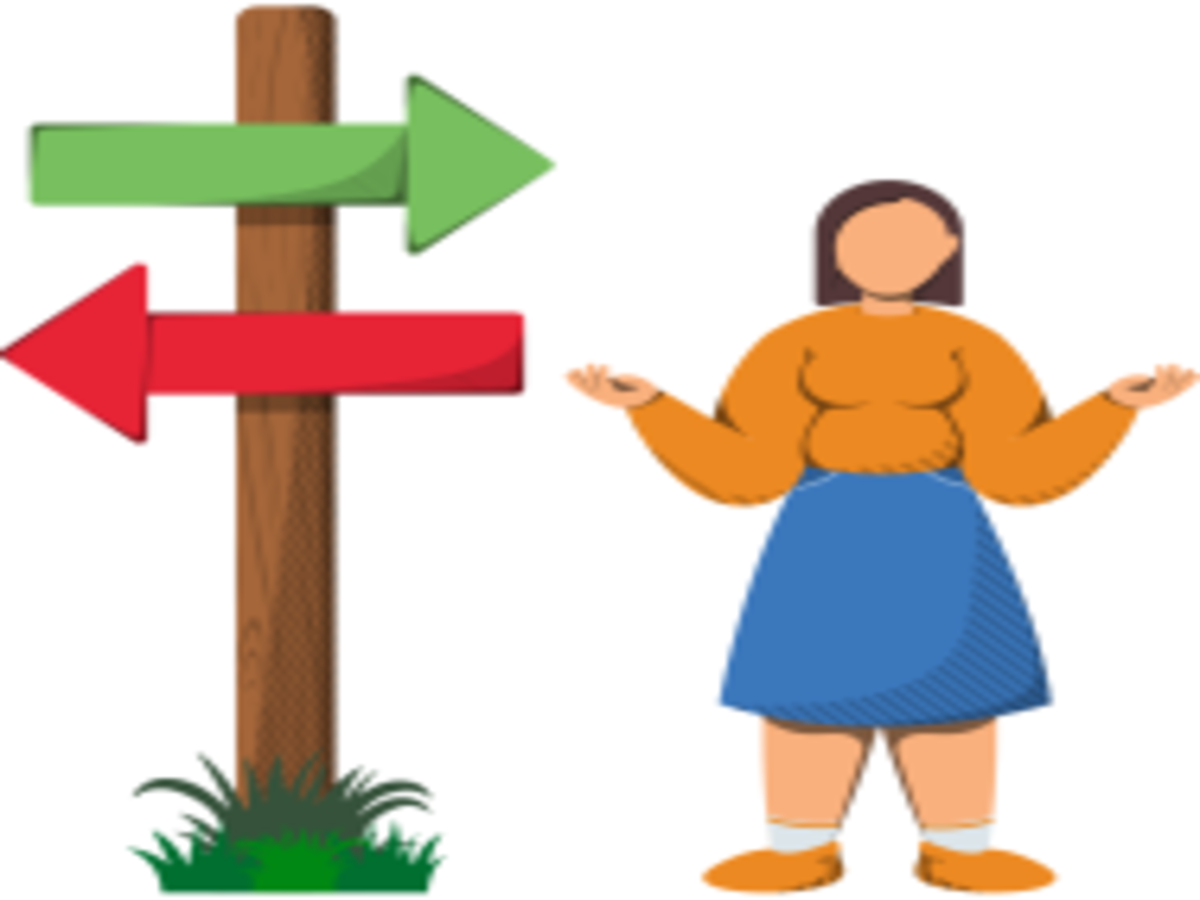
\includegraphics[width=0.8\textwidth]{Images/chapter_1/section_5546916426809344/6189662928764928.png}
\end{minipage}

For example, discussing whether to use the Room library instead of raw SQLite isn't helpful because the Room library is a mere wrapper around SQLite. A better discussion might be about using traditional databases like MySQL or NoSQL stores like MongoDB. The second discussion will help us pinpoint trade-offs between the two.

We should start with high-level stuff because the low-level details will automatically come up.

\subsection{Mock interviews}\label{_iBmPbw-jK71Gt4hITmkT}

\noindent
\begin{minipage}[t]{0.48\textwidth}
\textbf{Mock interviews} are a great way to prepare for System Design interviews. They involve pairing up with a friend and allowing them to ask questions. If it's not possible to use a friend, another strategy is to record ourselves and play the role of both interviewer and interviewee. With this approach, we can critique ourselves or ask a knowledgeable friend for feedback.
\end{minipage}
\hfill
\begin{minipage}[t]{0.48\textwidth}

\includegraphics[width=0.8\textwidth]{Images/chapter_1/section_5546916426809344/5008178058493952.png}
\end{minipage}

\begin{quote}
\textbf{Note:} It's a good idea to get experience by sitting in real interviews in tech companies. Once you've been through an interview or two, you'll be better able to evaluate what went right and what didn't. However, if you don\textquotesingle t have that opportunity, you can get a feel of a real interview by practicing with our personalized \href{https://www.educative.io/mock-interview}{System Design mock interviewer}.
\end{quote}

% End of section content